\documentclass{article}
\usepackage{graphicx} % Required for inserting images
\usepackage{amsmath}
\usepackage{amsfonts}
\usepackage{amssymb}
\usepackage{bm}
\usepackage{physics}
\usepackage{fancyhdr}
\usepackage{pgfplots}
\usepackage{siunitx}
\usepackage{braket}
\usepackage{mhchem}
\usepackage{chemfig}
\usepackage{gensymb}
\newcommand{\ve}{\mathbf}
\newcommand{\pa}{\partial}
\newcommand{\la}{\langle}
\newcommand{\ra}{\rangle}

\title{Fermi-Pasta-Ulam Problem}
\author{Lachlan Kan}
\date{March 2025}

\begin{document}
\maketitle
\section{Introduction}
Consider $N+1$ unit masses connected by springs of unit strength. We can write down the following 
Hamiltonian.
\begin{align}
    H=\frac{1}{2}\sum_{i=0}^Np_i^2+\frac{1}{2}\sum_{i=0}^N(x_{i+1}-x_i)^2
\end{align}
The boundary conditions are such that the "virtual points" $x_{N+1}=x_{-1}=0$. We will use this boundary condition for the remainder of this project. Notice that since we 
start counting from 0, our index goes up until $N$ and thus we end up with $N+1$
masses. Notice that for any $i$, there are two terms in the potential that concerns 
it. They are as follows 
\begin{align}
    (x_{i+1}-x_i)^2+(x_i-x_{i-1})^2
\end{align}
With this information,
 the equations of motion can be easily found via Hamilton's equations, where taking the 
 derivative with respect to $x_i$ amounts to focusing only on the segment from (2) that concerns the mass.  
\begin{align}
    \pdv{p_i}{t}&=-\pdv{H}{x_i}=x_{i+1}+x_{i-1}-2x_i\\ 
    \pdv{x_i}{t}&=\pdv{H}{p_i}=
    p_i 
\end{align}
Which leads to the following second order differential equation. 
\begin{align}
    \ddot{x}_i=x_{i+1}+x_{i-1}-2x_i
\end{align}
For each mass, we can ansatz a solution $x_i=A_ie^{j\omega t}$, where $j\equiv\sqrt{-1}$ and we
assume that they all share the same angular frequency $\omega$. Clearly this will only be the case when the system 
is oscillating in a normal mode. Hence we are solving for the normal modes. Using this ansatz, (5) becomes 
\begin{align}
    -\omega^2 A_i= A_{i+1}+A_{i-1}-2A_i
\end{align}
Writing out all the differential equations for $i=\{0,1,2,...,N\}$ and 
getting all the terms to one side, we obtain the following 
\begin{align}
    \begin{cases}
    0&=(\omega^2-2)A_0+A_{1}\\ 
    0&=A_0+(\omega^2-2)A_1+A_2\\   
    0&=A_1+(\omega^2-2)A_2+A_3\\ 
    \vdots \\
    0&= A_{N-1} +(\omega^2-2)A_N
    \end{cases}
\end{align}
This is now a linear system of equations with $N+1$ equations. 
To solve this, system, we must call upon linear algebra. Consider a vector with its component 
being that of the amplitudes. 
\begin{align}
    \ve{a}=
    \begin{bmatrix}
        A_0\\ 
        A_1\\ 
        \vdots\\ 
        A_{N-1}\\
        A_N
    \end{bmatrix}
\end{align}
Now we must construct the matrix. Notice that all the entries on the diagonal are 
$\omega^2-2$, since the coefficeints on $A_i$ is $\omega^2-2$. On their neighbours $A_{i-1}$ and $A_{i+1}$, 
the entries are all $1$. Hence, the matrix is 
\begin{align}
    \ve{M}=\begin{bmatrix}
        \omega^2-2\ \ \ \ \ \ \  1\ \ \ \ \ \ \ 0\ \ \ \ \ \ \ 0\ \dots\ 0\ \ \ \ \ \ \ 0\ \ \ \ \ \ \ 0\\ 
        1\ \ \ \ \ \ \ \omega^2-2\ \ \ \ \ \ \ 1 \ \ \ \ \ \ \ 0\ \dots\ 0\ \ \ \ \ \ \ 0\ \ \ \ \ \ \ 0\\
        0\ \ \ \ \ \ \ 1\ \ \ \ \ \ \ \omega^2-2 \ \ \ \ \ \ \ 1\ \dots\ 0\ \ \ \ \ \ \ 0\ \ \ \ \ \ \ 0\\
        \vdots\ \ \ \ \  \ \ \ \ \ \ \vdots \ \ \  \ \ \ \ \ \vdots \\ 
        0\ \ \ \ \ \ \ 0\ \ \ \ \ \ \ 0 \ \ \ \ \ \ \ 0 \ \ \ \ \dots\ 1\ \ \ \ \ \ \ \omega^2-2\ \ \ \ \ \ \ 1\\
        0\ \ \ \ \ \ \ 0\ \ \ \ \ \ \ 0 \ \ \ \ \ \ \ 0\ \ \ \ \dots\ 0\ \ \ \ \ \ \ 1\ \ \ \ \ \ \ \omega^2-2\\
    \end{bmatrix}
\end{align}
This is a discrete Laplacian matrix of the tridiagonal form. Now, the system of (7) reduces to the following vector equation 
\begin{align}
    \ve{M}\ve{a}=\ve{0}
\end{align}
Or, equivalently expanded, we have the following 
\begin{align}
    \begin{bmatrix}
        \omega^2-2\ \ \ \ \ \ \  1\ \ \ \ \ \ \ 0\ \ \ \ \ \ \ 0\ \dots\ 0\ \ \ \ \ \ \ 0\ \ \ \ \ \ \ 0\\ 
        1\ \ \ \ \ \ \ \omega^2-2\ \ \ \ \ \ \ 1 \ \ \ \ \ \ \ 0\ \dots\ 0\ \ \ \ \ \ \ 0\ \ \ \ \ \ \ 0\\
        0\ \ \ \ \ \ \ 1\ \ \ \ \ \ \ \omega^2-2 \ \ \ \ \ \ \ 1\ \dots\ 0\ \ \ \ \ \ \ 0\ \ \ \ \ \ \ 0\\
        \vdots\ \ \ \ \  \ \ \ \ \ \ \vdots \ \ \  \ \ \ \ \ \vdots \\ 
        0\ \ \ \ \ \ \ 0\ \ \ \ \ \ \ 0 \ \ \ \ \ \ \ 0 \ \ \ \ \dots\ 1\ \ \ \ \ \ \ \omega^2-2\ \ \ \ \ \ \ 1\\
        0\ \ \ \ \ \ \ 0\ \ \ \ \ \ \ 0 \ \ \ \ \ \ \ 0\ \ \ \ \dots\ 0\ \ \ \ \ \ \ 1\ \ \ \ \ \ \ \omega^2-2\\
    \end{bmatrix}\begin{bmatrix}
        A_0\\ 
        A_1\\ 
        A_2\\
        \vdots\\ 
        A_{N-1}\\
        A_N
    \end{bmatrix}
    =
    \begin{bmatrix}
        0\\ 
        0\\ 
        0\\
        \vdots\\ 
        0\\
        0
    \end{bmatrix}
\end{align}
To solve this, we take the determinant of $\ve{M}$ and set it to 0. Then we can solve 
for $\omega$ directly. This method is easily implementable on python. However, it 
is computationally expensive and the computation time 
gets much longer with every mass added to the chain. 

\section{Nonlinear Perturbation}
We now perturb the spring potential by a nonlinear term. Let $\alpha$ be a small 
positive number. The new Hamiltonian is therefore 
\begin{align}
    H=\frac{1}{2}\sum_{i=0}^Np_i^2+\frac{1}{2}\sum_{i=0}^N[  (x_{i+1}-x_i)^2 + \alpha (x_{i+1}-x_i)^\gamma ]
\end{align}
Where $\gamma=2$ or 3, depending on whether the perturbation is quadratic or cubic. Applying the same Hamilton equations, we arrive at the following equations of motion 
\begin{align}
    \dot{p_i}&=(x_{i+1}+x_{i-1}-2x_i)+\alpha [(x_{i+1}-x_i)^\gamma-(x_i-x_{i-1})^\gamma]\\
    \dot{x_i}&=p_i
\end{align}
Here, we are interested in solving directly for the equations of motion. For computational purposes, 
it is best to condense all the momenta and position equations of the particles
into one state vector
\begin{align}
    \ve{v}=\begin{bmatrix}
        p_0\\ 
    x_0\\ 
    p_1\\ 
    x_1\\ 
    \vdots\\ 
    p_N\\ 
    x_N
    \end{bmatrix}
\end{align}
If we denote $\ve{v}=v^\mu$ where $\mu=\{ 0, 1, 2, ..., 2N\}$, 
then an even $\mu$ denotes momenta  and an odd $\mu$ denotes position.
From (15), we can specify the initial conditions by specifying $\ve{v}(0)$.
Similarly, we can construct a vector 
that encodes the time evolution of the state vector 
\begin{align}
    \dot{\ve{v}}=\begin{bmatrix}
    \dot{p}_0\\ 
    \dot{x}_0\\ 
    \dot{p}_1\\ 
    \dot{x}_1\\ 
    \vdots\\ 
    \dot{p}_N\\ 
    \dot{x}_N\\ 
    \end{bmatrix}
\end{align}
Where the time derivatives $\dot{p}_i$ and $\dot{x}_i$ can be found in (13) and (14) respectively. In Python, 
we can solve the system by creating a function that generates the evolution vector, 
and then passing the function (not the evolution vector itself, but the function that generates it), as well as the initial conditions 
$\ve{v}(0)$ on to 
scipy for solving. Since there is a nonlinear term to the differential equations, 
it is best to choose the Backwards Differentiation Formula (BDF) method to solve the system. 
A way to check for correctness of the code is to use only two masses and set 
$\alpha=0$. We can then 
displace the masses identically and release from rest. If this results in a normal mode, then the code is likely to be correct.

\section{Modal Spectra}
The mode spectra of the FPU oscillator can be found as the Fourier sine 
transform of the displacement. The discrete Fourier coefficient $\phi_{ik}$ for the 
$i-$th particle in the $k$-th mode is well known to be 
\begin{align}
    \phi_{ki}=\sqrt{\frac{2}{N}}\sin\frac{ik\pi}{N}
\end{align}
We can thus construct the matrix $\phi_{ki}$ where the rows represent modes and 
columns represent particles. If we extract only the displacement from the state vector
and write out all its time evlolution on the rows, then we obtain 
\begin{align}
    d_{it}=\begin{bmatrix}
        x_0(0)& x_0(t_1) & x_0(t_2) &\cdots \ \  x_0(t_f)\\ 
        x_1(0)& x_1(t_1) & x_1(t_2) &\cdots \ \  x_1(t_f)\\ 
       \vdots& \vdots & \vdots & \vdots\\ 
        x_N(0)& x_N(t_1) & x_N(t_2) &\cdots \ \ x_N(t_f)\\ 
    \end{bmatrix}
\end{align} 
We can thus find the discrete sine transform via the following well known formula 
\begin{align}
    a_{kt}=\sqrt{\frac{2}{N}}\sum_ix_i(t)\sin{\frac{ik\pi}{N}}
\end{align}
Notice the $t$ in the subscript means that we must apply the transformation across 
all time. Notice that we sum across all $i$, and 
$i$ is an index that appears in both $d_{it}$ and $\phi_{ik}$. This "summing over repeated index"
is equivalent to the matrix product.
 Hence, the Fourier coefficeints for every point in time $t$ can be found by 
the following product 
\begin{align}
    a_{kt}=\phi_{ki}d_{it}
\end{align}
This can be easily calculated in Python by the $@$ operator, and has components of the time 
evolution of each mode. We can easily find the momenta modes by constructing the same matrix 
in (18) but with momenta, and projecting that onto the basis matrix $\phi_{ki}$, which yields 
the Fourier sine transform of momenta.

\subsection{Excitatation of Modes}
To excite a certain mode, say the $k$-th mode, all we have to do is initialise the state vector 
in a way such that 
the initial displacement matches up exactly with the Fourier coefficient $\phi_{ki}$ for the 
$i$-th particle in that $k$-th mode. When the initial conditions are set up this way, the mode spectra 
will show a large amplitude for the desired mode $k$ and very low (zero) amplitudes for the other modes.
However, it has been found that if the initial conditions deviate from the expected $\phi_{ki}$ 
even for just a littile bit, the amplitude will "spread" from 
the $k$-th mode to the other modes, resulting in high amplitudes in the other modes over time.
\section{Results}
Here are some results and examples from the Python code, implementing the methods outlined in the previous sections.
\subsection{Quadratic Perturbation}
Here we will demonstrate the results when $\gamma=2$, which corresponds to the FPU-$\alpha$ problem.
\subsubsection{Testing with a Known Case}
To test the code, we first run it with $\alpha=0$ (no nonlinearity - a known case) with two masses 
starting with equal displacement. We obtain figure 1.
Notice that their displacements are identical. We have reached a normal mode. This is 
a known case, and we can be more confident that our solver is correct.
\subsubsection{Four Masses}
We can now examine more interesting cases. Consider 4 masses under quadratic perturbation. 
Here we have set $\alpha=1/6$ and displaced them initially with slightly different displacements, as shown in figure 2.
\subsection{Fifty Masses}
We will test 50 masses displaced identically at the start, released from rest. The plot, 
shown in figure 3 is beginning to look 
like that of a continuum. The small plot however, does not do the system justice since 
its amplitudes of oscillation are somewhat muted due to the sheer volume of masses needed 
to be fit into the small plot.
\subsection{Mode Spectra}
Here we will deal with the mode spectra part of the simulation.
\subsubsection{Exciting the First Mode}
Here, we will initialise the initial 
conditions such that they match up with the $k=1$ mode. 
Again, we will be dealing with 4 masses and testing with no nonlinearity. This results in 
figure 4. Notice that all other modes are 0 except for the $k=1$ mode. This is what we expect. 
We can now see what happens when there exists some nonlineariy, say $\alpha=1/4$. This results in 
figure 5. Notice that immediately, some Fourier amplitude gets "transferred" into the second mode. 
\subsection{Arbitrary Initial Conditions}
Here we will impose upon the system of 4 masses an arbitrary set of initial conditions, with $\alpha=1/4$ and 
observe the behaviour. This results in figure 6. Notice that one mode still dominates over the other, however 
the oscillations are now a combination of the modes.
\subsection{The Paradox}
In the modal spectra plots, we see that the first (excited) mode gradually decreases
in Fourier amplitude and the rest has its Fourier amplitudes gradually increase.
It may be tempting the think that if we let the simulation run long enough, that there will 
be a stable point where all the modes balance and the Fourier amplitudes do not change. In oter words, 
the system will thermalise. However, our results shown in figure 7 tells a different story. Here, 
we run a much longer and large scale simulation, with $\alpha=0.6$ and 32 masses for a max time of 
36000 to observe the long term behaviour of the system. 
We also start the simulation by imposing initial conditions that excite the mode $k=1$. 
 we observe the classic FPU paradox - 
instead of reaching equilibrium, the modes oscillate. For example, mode 1 starts decreasing and 
mode 2 increases, but after sufficient time, mode 2 will start decreasing and mode 1 will increase again. 
This periodic behaviour was the original paradox, discovered by Fermi, Pasta and Ulam. 
In this simulation, the maximum Fourier amplidue for mode 1 decreases every major cycle.
This raises the question of whether or not there is a bigger cycle, or does 
the system truly thermalise for large enough times.
Unfortunately, this simulation was already heavy for the Macbook and the system is 
nowhere near thermalising. Thus we can only conclude that even if the system thermalises,
 the timescales required is too large to simulate on a typical computer. 


\section{Figures}
\begin{center}
    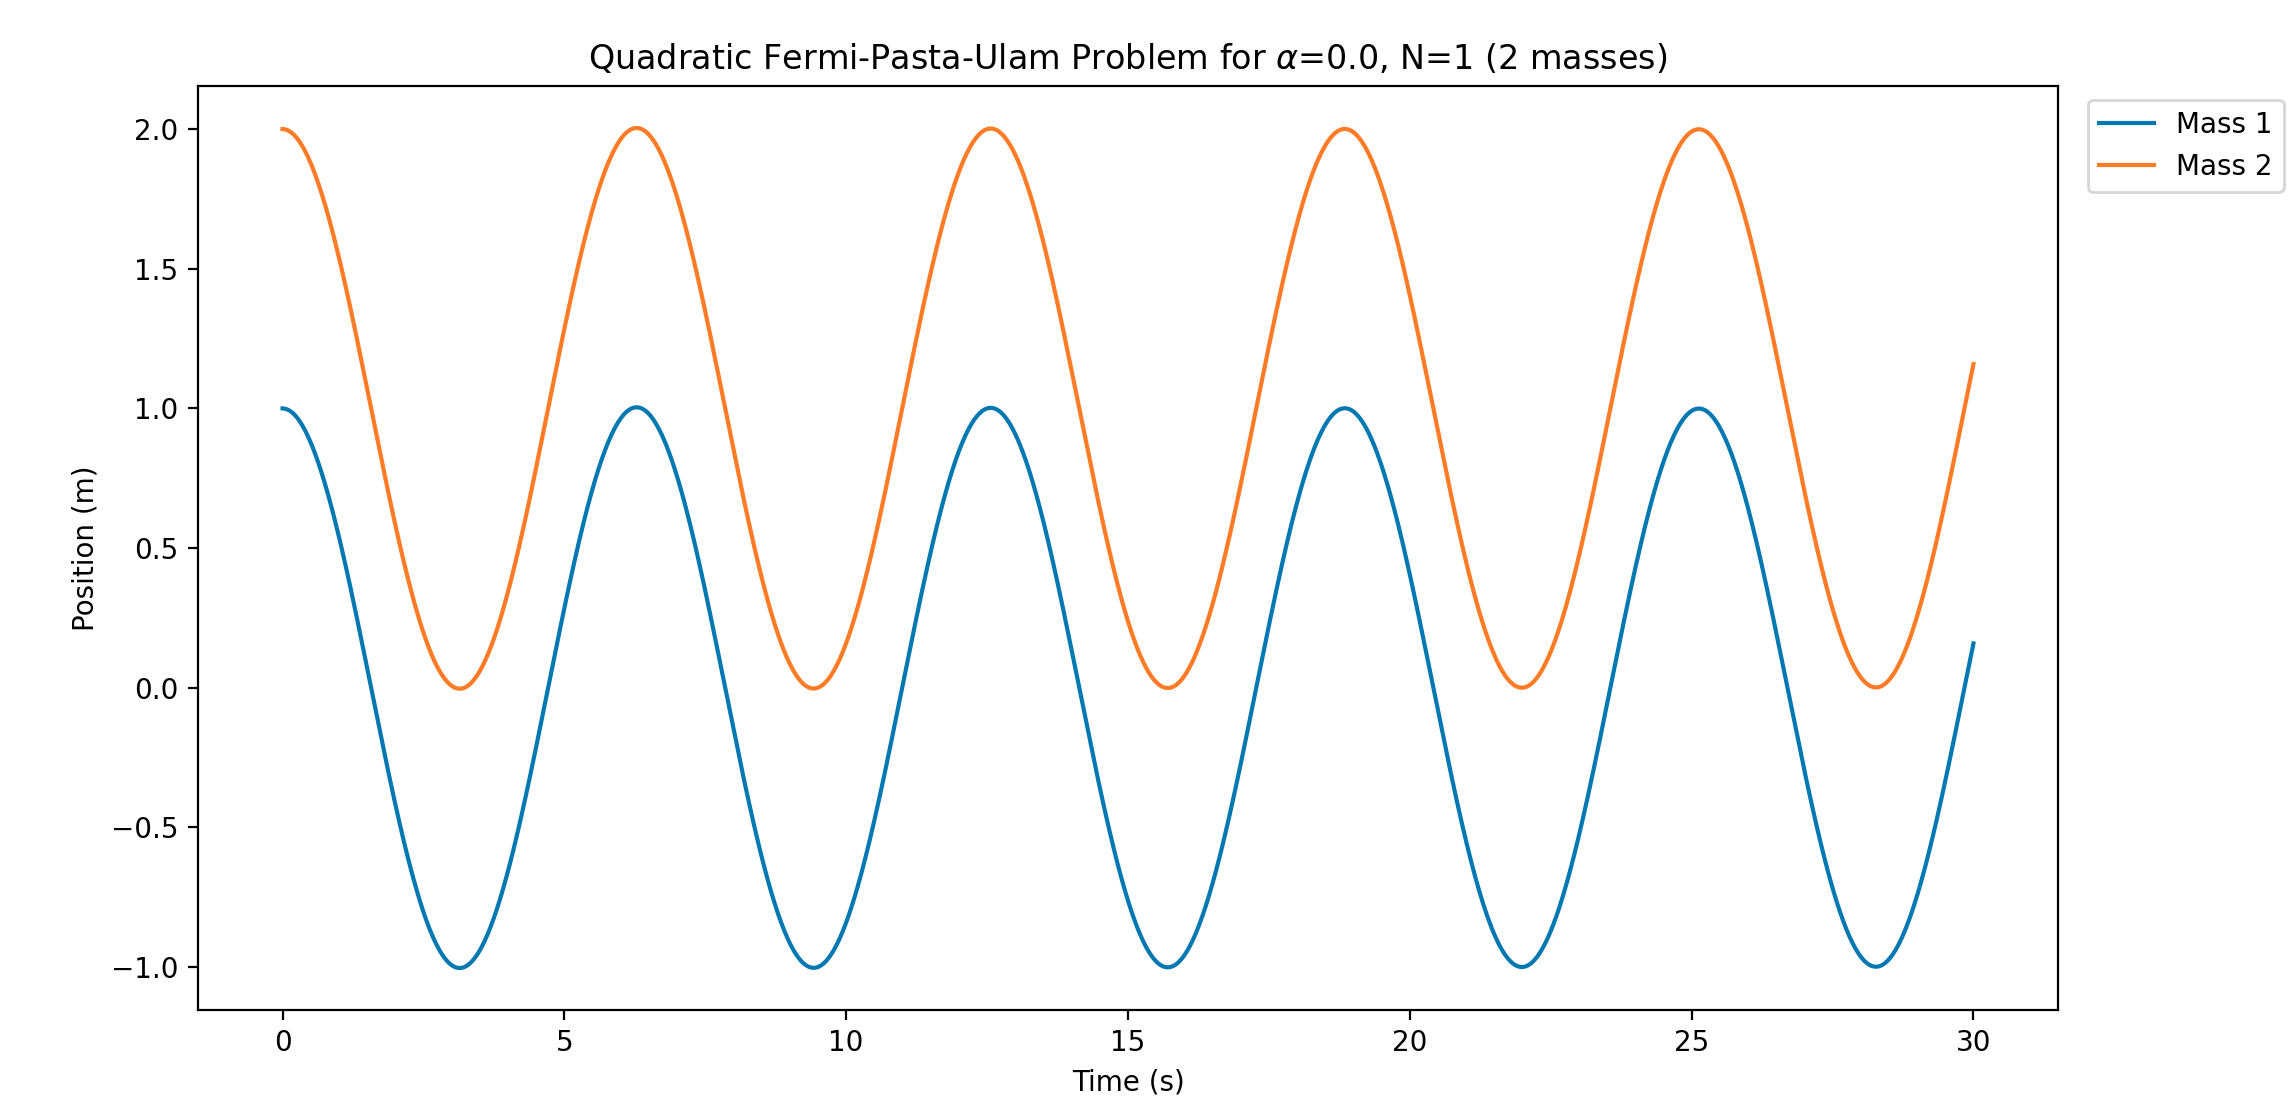
\includegraphics[scale=.33]{2mass.png}\\ 
    (Fig. 1)\\ 
    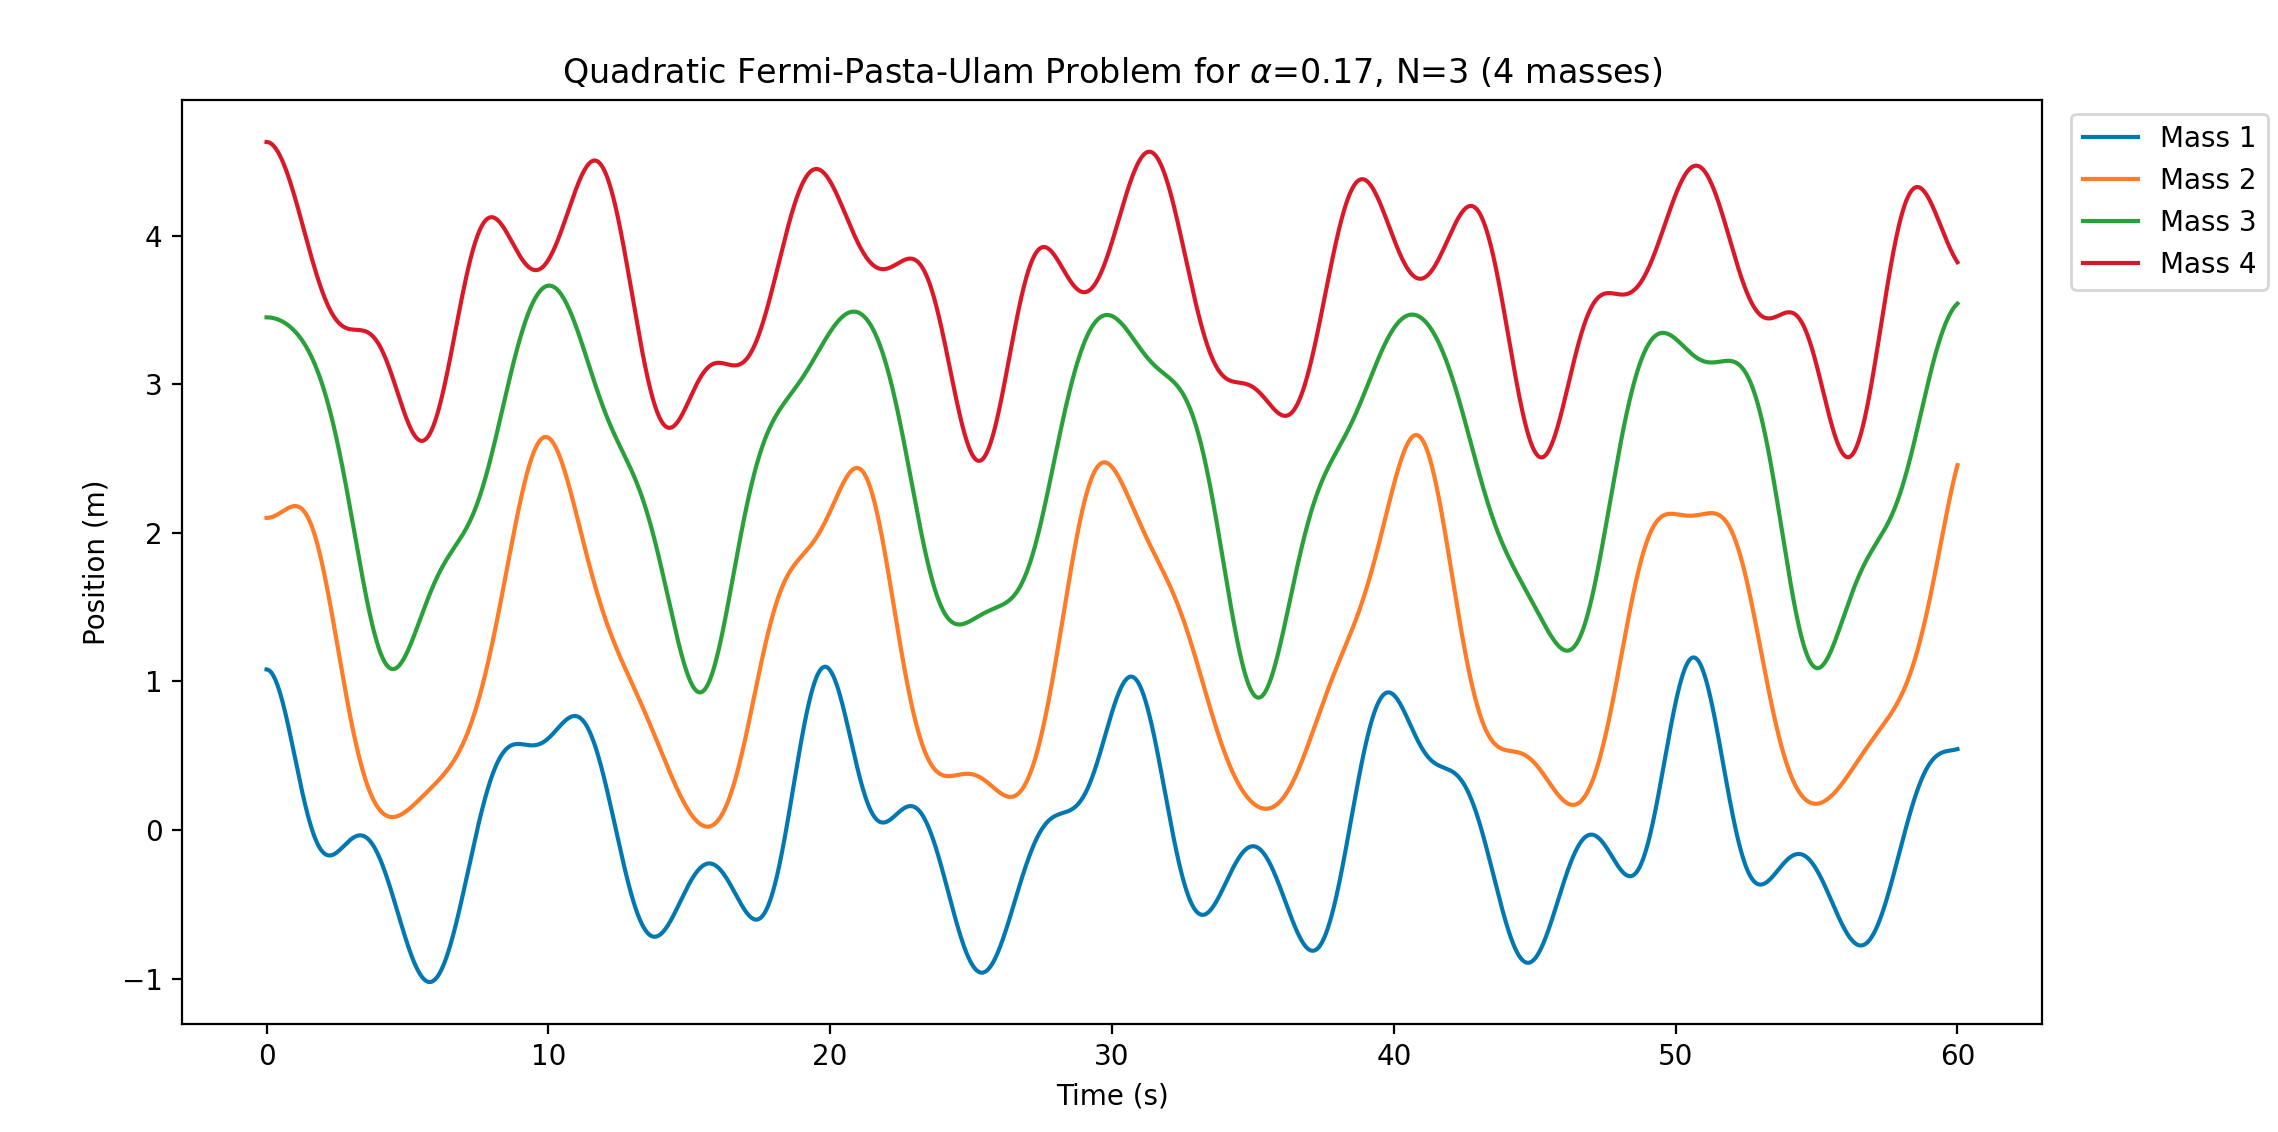
\includegraphics[scale=.33]{4mass.png}\\ 
    (Fig. 2)\\ 
    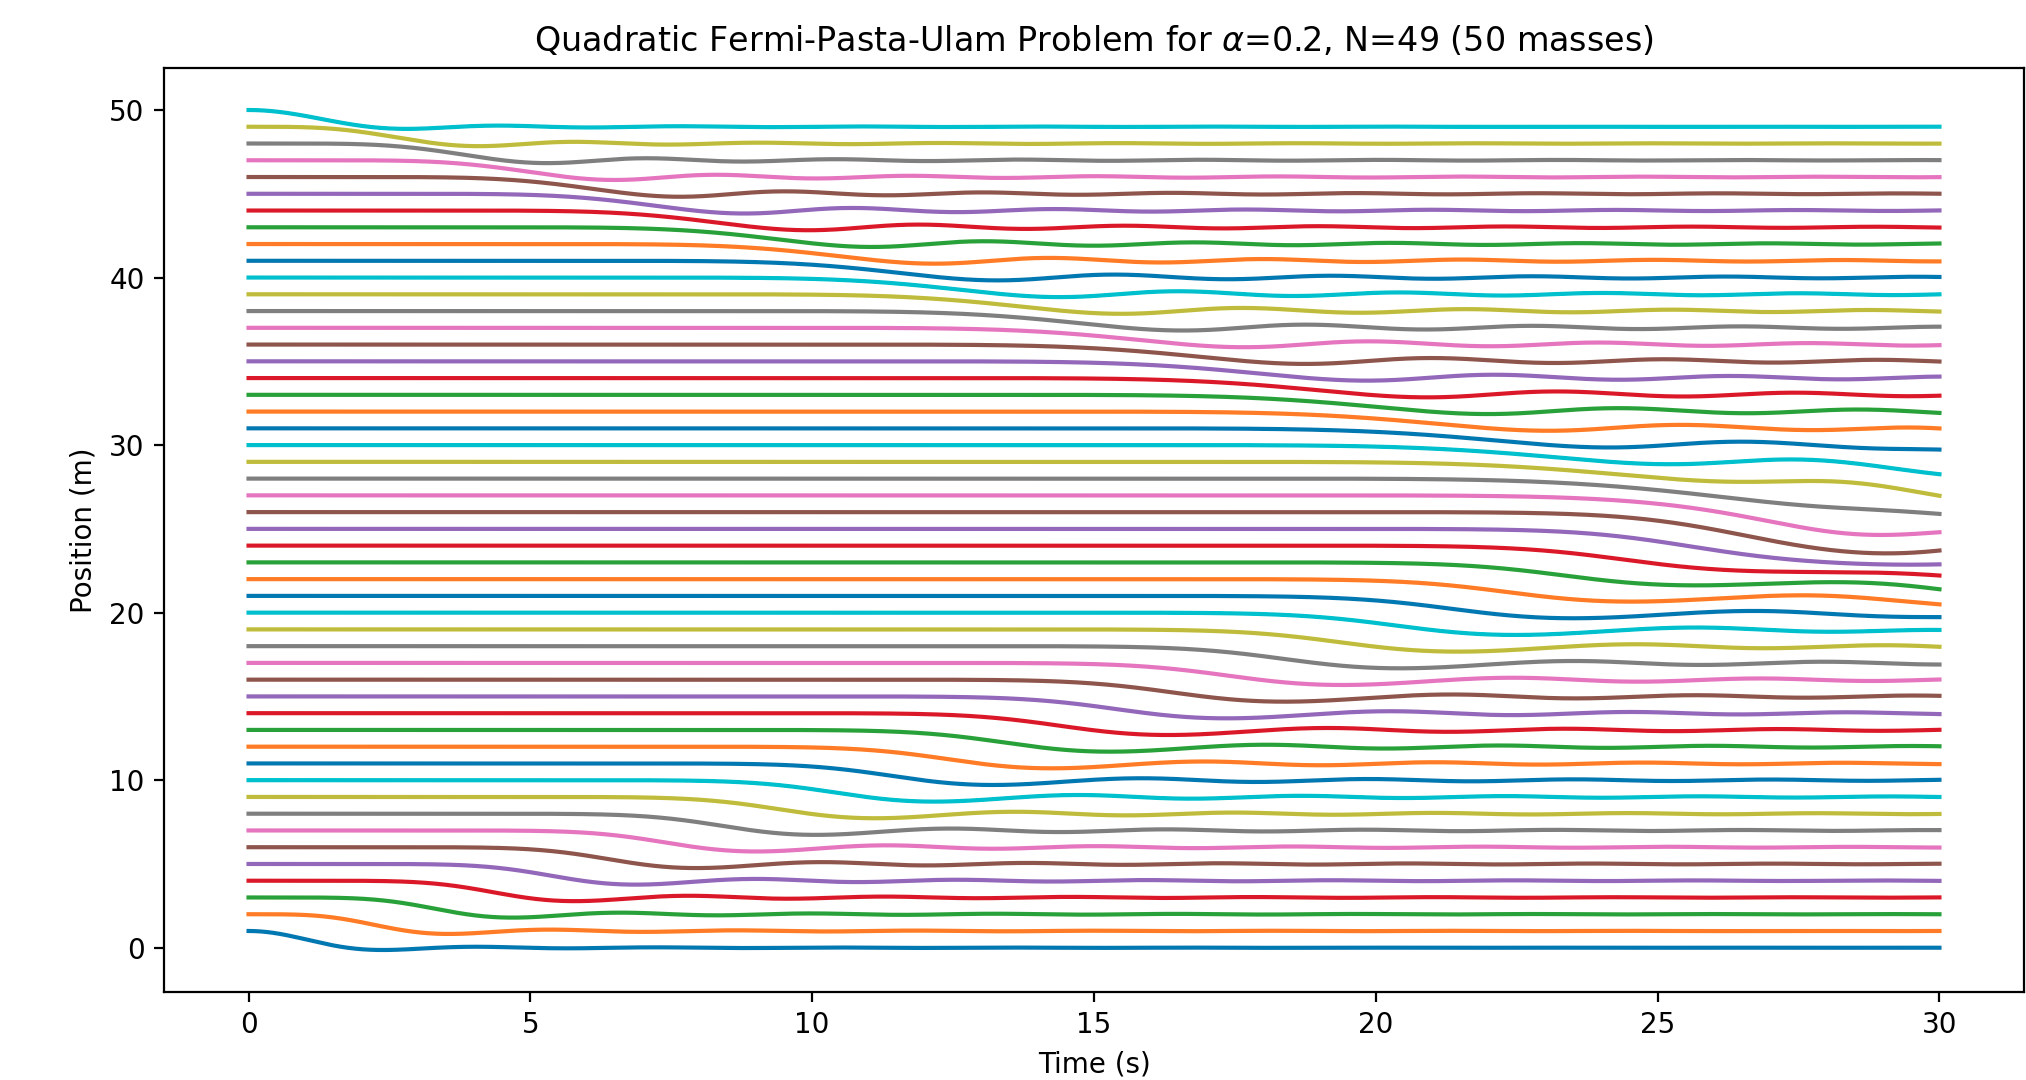
\includegraphics[scale=.33]{50mass.png}\\ 
    (Fig. 3)\\ 
    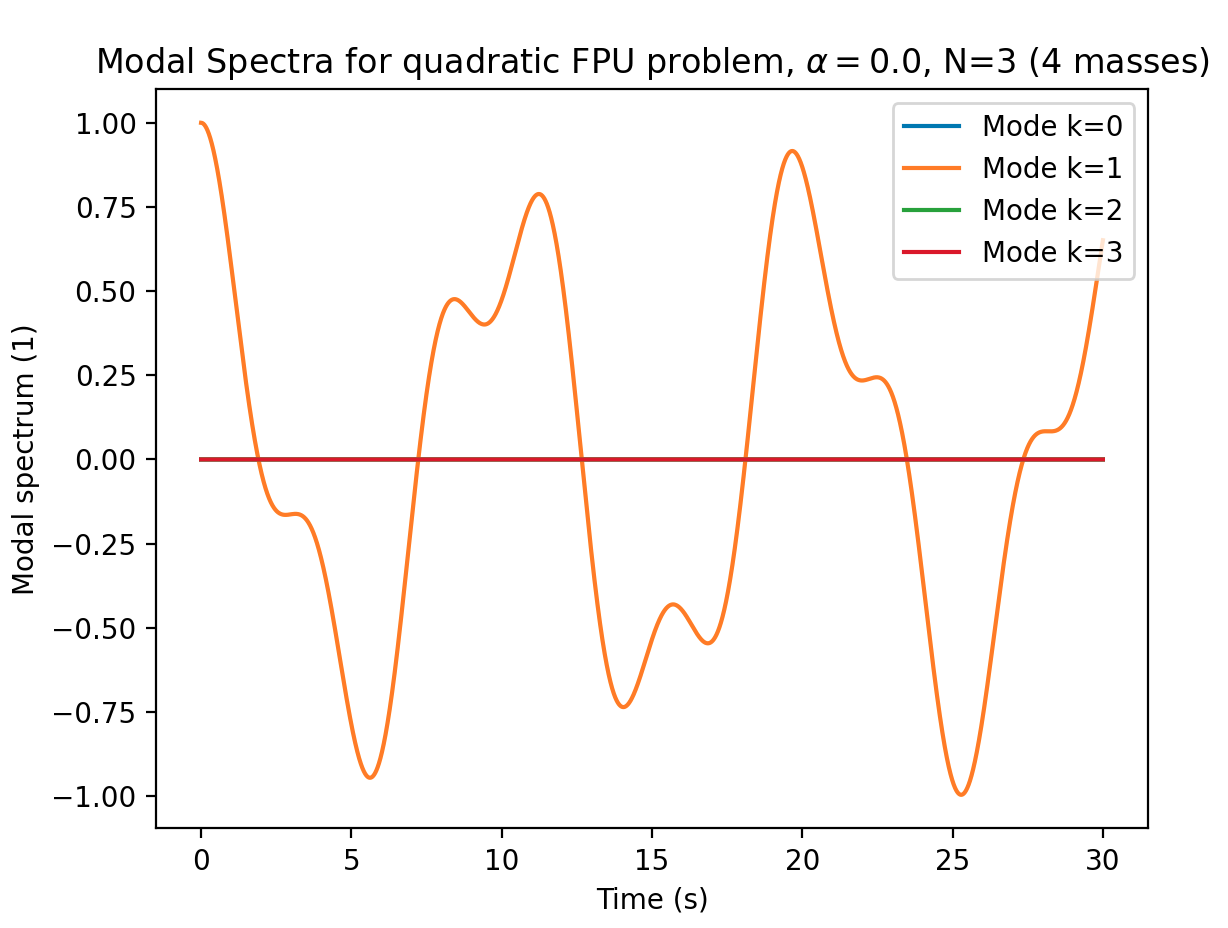
\includegraphics[scale=.5]{modea0k1.png}\\ 
    (Fig. 4)\\ 
    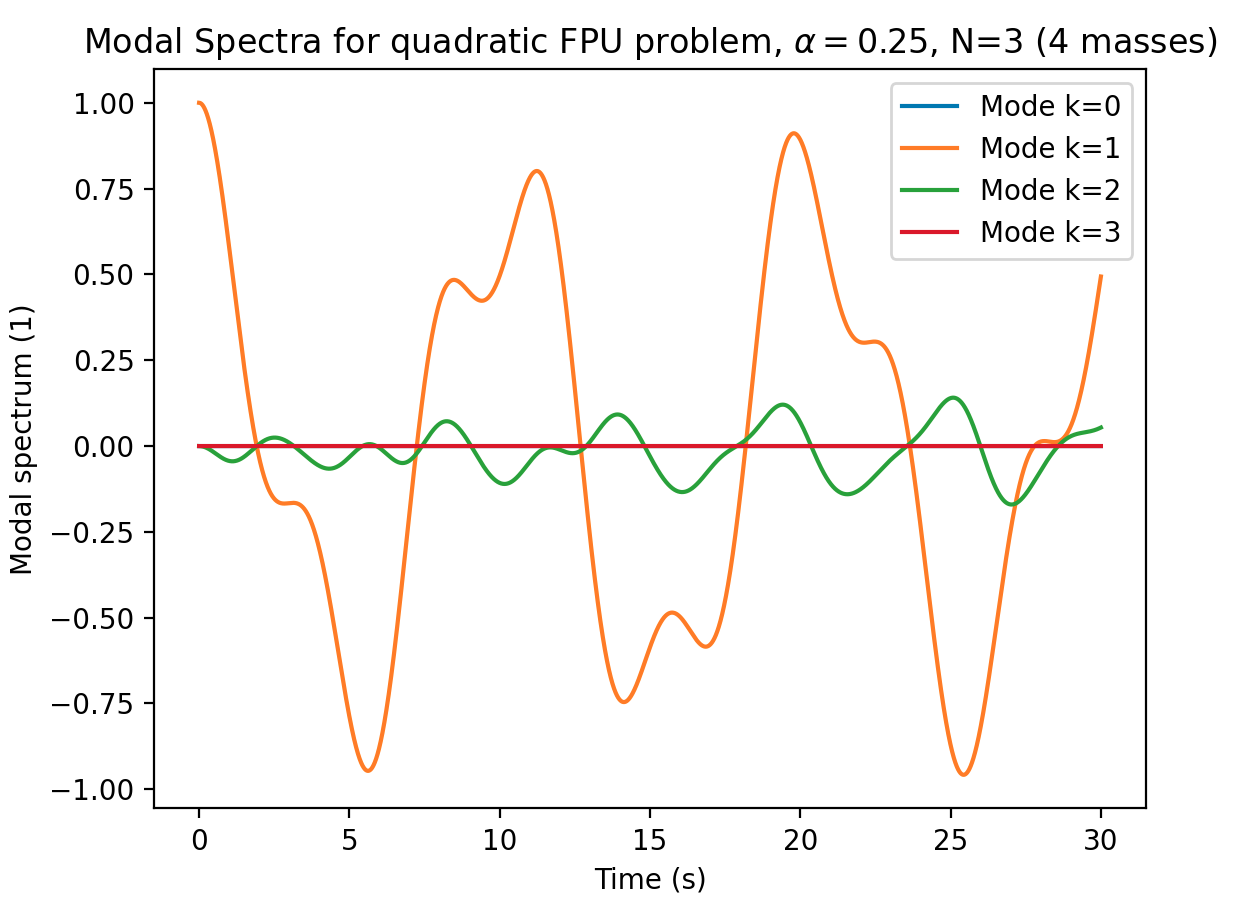
\includegraphics[scale=.5]{modea25k1.png}\\ 
    (Fig. 5)\\ 
    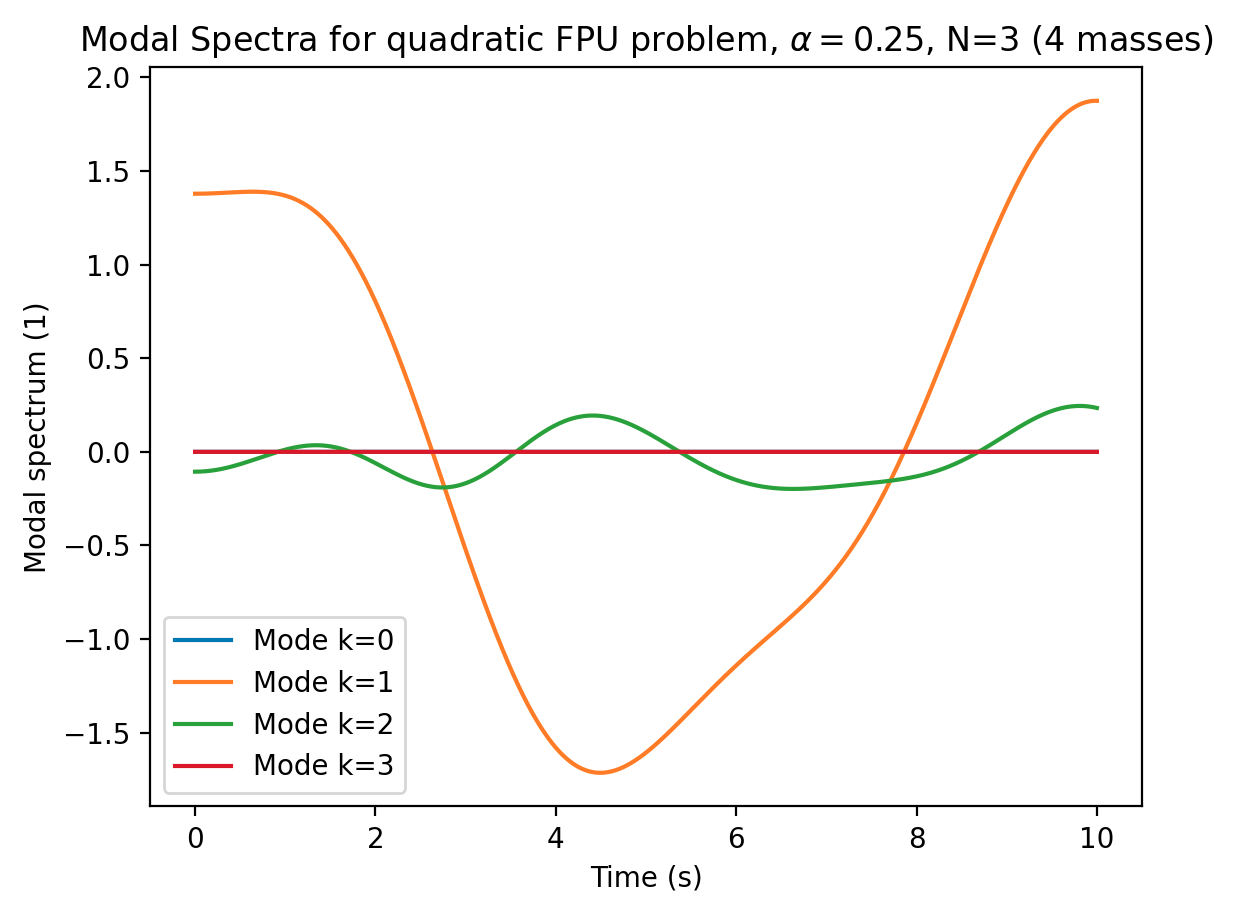
\includegraphics[scale=.5]{modea25arb.png}\\ 
    (Fig. 6)\\ 
    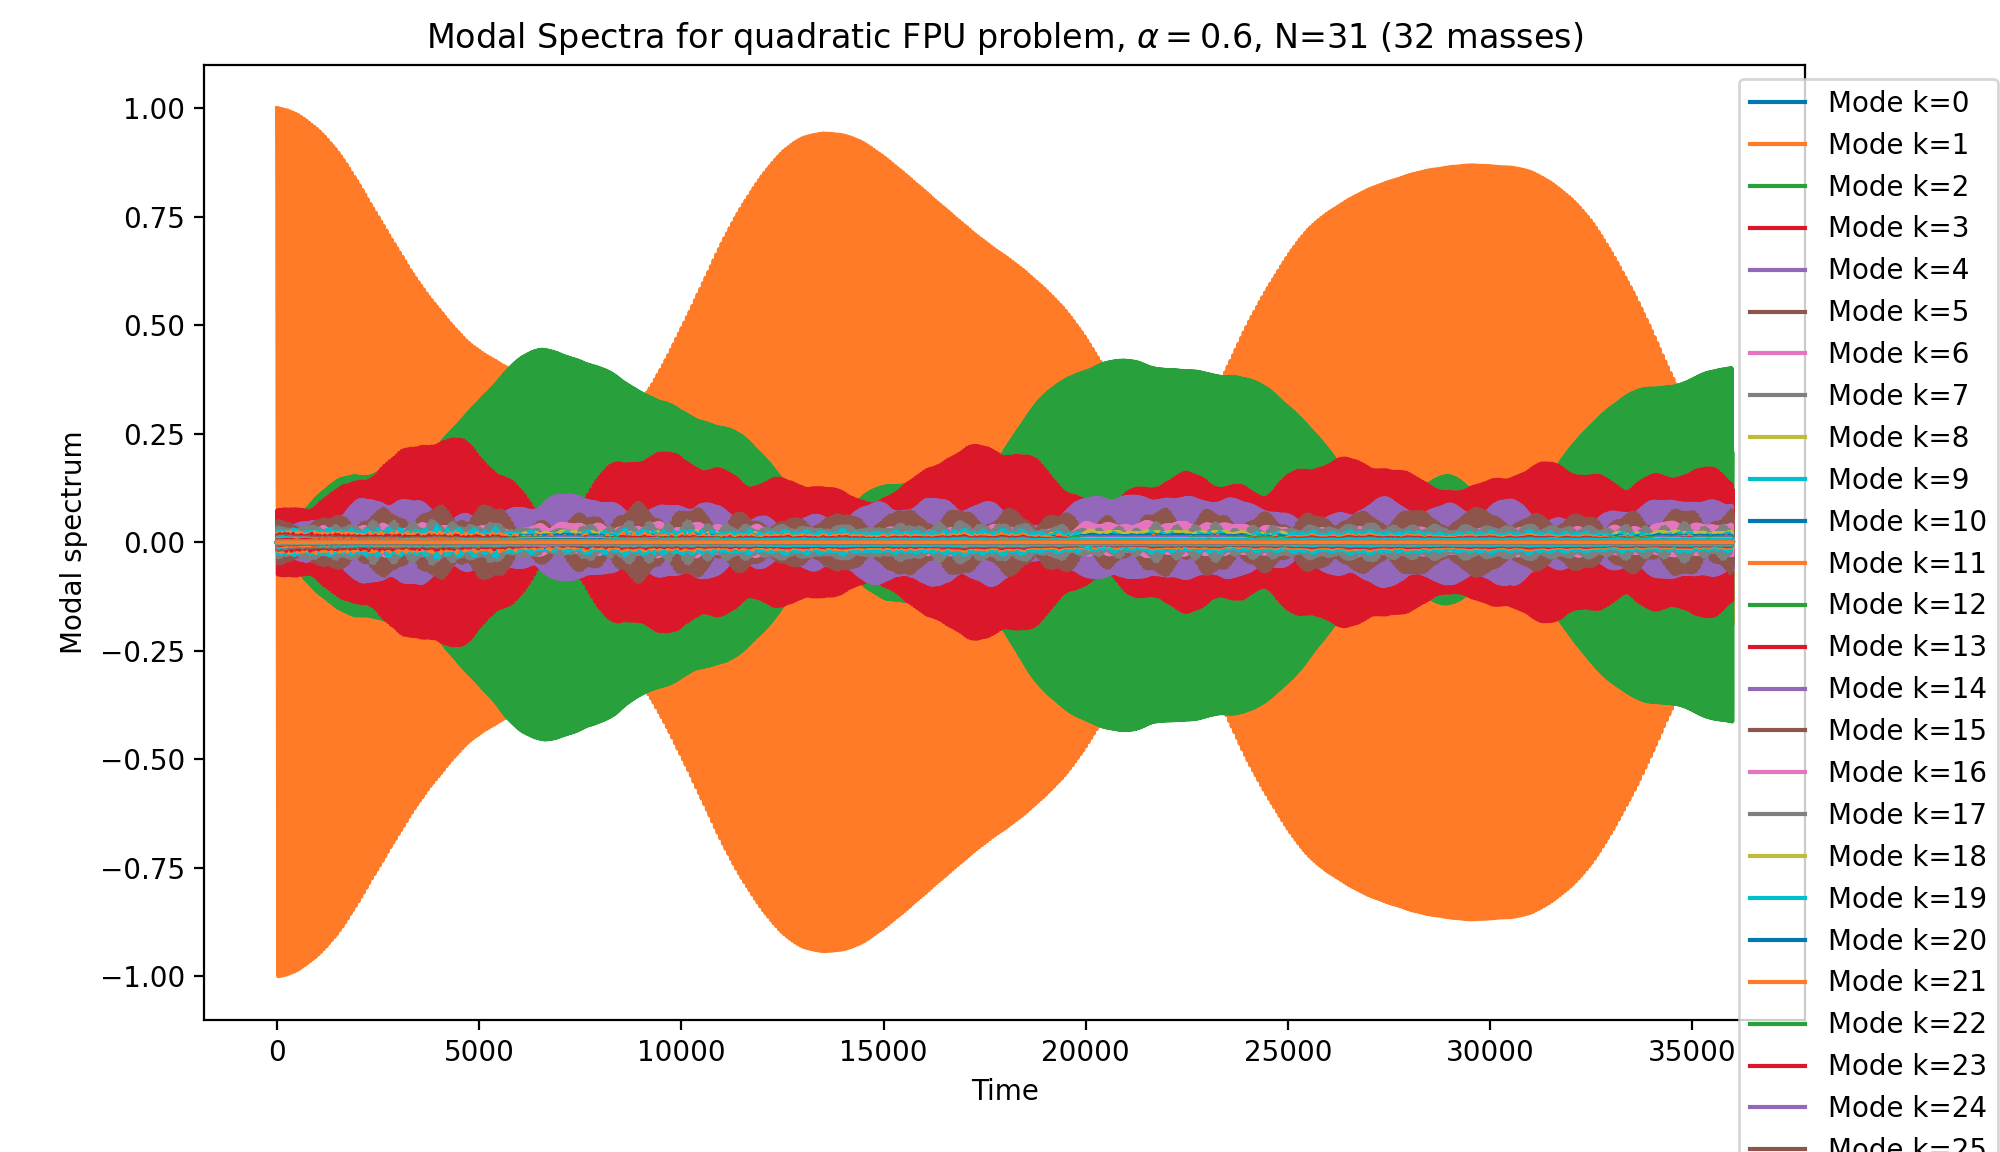
\includegraphics[scale=.36]{modea6k1.png}\\ 
    (Fig. 7)
\end{center} 
\end{document}
